%\documentclass[11pt,draftcls,onecolumn]{IEEEtran}
\documentclass[10pt,twocolumn]{IEEEtran}
\newcommand{\fv}{\mbox{\boldmath $f$}}
\newcommand{\Iv}{\mbox{\boldmath $I$}}
\newcommand{\xv}{\mbox{\boldmath $x$}}
\newcommand{\velocity}{\mbox{\boldmath $v$}}
\newcommand{\velocityinv}{\mbox{\boldmath $v$}^{-1}}
\newcommand{\Velocityinv}{\mbox{\boldmath $V$}^{-1}}
\newcommand{\Velocity}{\mbox{\boldmath $V$}}
\newcommand{\welocity}{\mbox{\boldmath $w$}}
\newcommand{\spatialimagegradient}{\mbox{\boldmath $I$}\mbox{$_{x}$}}
\newcommand{\perpspatialimagegradient}{\mbox{\boldmath $I$}\mbox{$^{\perp}_{x}$}}
\newcommand{\temporalimagederivative}{\mbox{$I_t$}}
\newcommand{\finitestrain}{\mbox{\boldmath $\varepsilon^{\ast}$}}
\newcommand{\smallstrain}{\mbox{\boldmath $\varepsilon$}}
\newcommand{\dispgradient}{{\bf \nabla \displace}}
\newcommand{\displace}{{\bf u}} 
\newcommand{\Id}{\text{\bf Id}}
\newcommand{\ode}{{\em O.D.E.}}
\newcommand{\odes}{{\em O.D.E.}s}
\newcommand{\G}{\mathcal{G}}
\newcommand{\J}{\mathcal{J}}
\newcommand{\phiinv}{\phi^{-1}}
\newcommand{\psiinv}{\psi^{-1}}
\newcommand{\dM}{DM}
\newcommand{\DM}{Diffeomorphometry}
\newcommand{\diff}{diffeomorphism}
\newcommand{\Diff}{Diffeomorphism}
\newcommand{\orbit}{\mathcal{O}}
\newcommand{\avg}{\mathcal{A}}
\newcommand{\avgn}{\mathcal{A}_n}
\newcommand{\avgna}{\mathcal{A}^a_{n}}
\newcommand{\nset}{\{ J_i \}_n}
\newcommand{\bari}{\bar{I}}
\newcommand{\bart}{\bar{t}}
\newcommand{\jac}{\mathcal{J}}
\newcommand{\pert}{\mbox{\boldmath $w$}}
\newcommand{\barpert}{\bar{\mbox{\boldmath $w$}}}
\newcommand{\half}{0.5}
\newcommand{\X}{{\bf X}}
\newcommand{\x}{{\bf x}}
\newcommand{\Z}{{\bf Z}}
\newcommand{\z}{{\bf z}}
\newcommand{\p}{{\bf p}}
\newcommand{\Y}{{\bf Y}}
\newcommand{\y}{{\bf y}}
\newcommand{\ytild}{\tilde{{\bf y}}}
\newcommand{\q}{{\bf q}}
\newcommand{\surf}{\mathcal{S}}
\newcommand{\phij}{\phi_{ij}}
\newcommand{\aphij}{\bar{\phi}_{j}}
\newcommand{\apsij}{\bar{\psi}_{j}}
\newcommand{\aphi}{\bar{\phi}}
\newcommand{\aphiinv}{\bar{\phi}^{-1}}
\newcommand{\domain}{\Omega}
\newcommand{\meanshape}{\bf \bar{x}}
\newcommand{\g}{\mbox{\boldmath $g$}}
\newcommand{\h}{\mbox{\boldmath $h$}}
\newcommand{\yv}{\mbox{\boldmath $y$}}
\newcommand{\group}{Diff}
\newcommand{\evol}{{E_{\text{Vol}}}}
\newcommand{\epair}{{E_{\text{Pair}}}}
\newcommand{\esec}{{E_{S}}}
\newcommand{\inv}{^{-1}}
\newcommand{\vinit}{ \velocity^0_{ij}(\x,\tau=0) }
\newcommand{\avinit}{ \bar{\velocity}^0_{j}(\x,t) }
\newcommand{\avinitz}{ \bar{\velocity}^0_{j}(\x,t_a) }
\newcommand{\gz}{\nabla_{\z}}
\newcommand{\Section}[1]{\vspace{-8pt}\section{\hskip-1em.~~#1}\vspace{-3pt}}
\newcommand{\SubSection}[1]{\vspace{-3pt}\subsection{\hskip -1em.~~#1}\vspace{-3pt}}
\newcommand{\BASE}{.}%/Users/stnava/Work/}
\newcommand{\TEXDIR}{.}%{\BASE Words/Writing/}
\newcommand{\ROOT}{.}%{\BASE Words/}
\newcommand{\FIGDIR}{.}%{\BASE Words/Writing/MEDIAITK/wbir/}
\newcommand{\FIGDIRAIBS}{.}%{\BASE Words/Writing/IPMI2003/jpegs/}
\newcommand{\FIGDIRP}{proposal/}%{\BASE Words/Writing/proposal/}
\newcommand{\FIGDIRPJ}{proposal/jpegs/}%{\BASE Words/Writing/proposal/jpegs/}
\newcommand{\FIGDIRADAD}{.}%{\BASE Words/Writing/ADAD/}
\newcommand{\FIGS}{.}%{\BASE Words/Writing/neuroimageipam-final/FIGS/}
%
% This example can be formatted using the peerreview
% (instead of journal) mode.
%\documentclass[11pt,draftcls,onecolumn]{IEEEtran}
\usepackage{amssymb,amsmath}
\usepackage{color}
\usepackage{algorithm}
\usepackage{algorithmic}
\usepackage{rotating}
\usepackage{multirow,booktabs,ctable,array}
\usepackage{listing}						
\usepackage{listings}					
\graphicspath{./Figures/}
\hyphenation{op-tical net-works semi-conduc-tor}
\usepackage{lineno}
\begin{document}
\definecolor{listcomment}{rgb}{0.0,0.5,0.0}
\definecolor{listkeyword}{rgb}{0.0,0.0,0.5}
\definecolor{listbackground}{gray}{0.965}
\lstset{frame = tb,
        framerule = 0.25pt,
        float,
        fontadjust,
        backgroundcolor={\color{listbackground}},
        basicstyle = {\ttfamily\scriptsize},
        keywordstyle = {\ttfamily\color{listkeyword}\textbf},
        identifierstyle = {\ttfamily},
        commentstyle = {\ttfamily\color{listcomment}\textit},
        stringstyle = {\ttfamily},
        showstringspaces = false,
        showtabs = false,
        numbers = none,
        tabsize = 2,
        language=[ISO]C++,
        floatplacement=!h
        }	



%
% paper title
\title{ANTS: Open-Source Tools for Normalization And Neuroanatomy}
%
%
% author names and IEEE memberships
% note positions of commas and nonbreaking spaces ( ~ ) LaTeX will not break
% a structure at a ~ so this keeps an author's name from being broken across
% two lines.
% use \thanks{} to gain access to the first footnote area
% a separate \thanks must be used for each paragraph as LaTeX2e's \thanks
% was not built to handle multiple paragraphs
\author{Brian B. Avants, Nicholas J. Tustison, Gang Song, and James C. Gee
%               Penn Image Computing and Science Laboratory \\
%               University of Pennsylvania \\
%               3600 Market Street, Suite 370 \\
%               Philadelphia,  PA  19104 \\
%               contact email:  tustison@grasp.cis.upenn.edu
%\thanks{Manuscript received XXX; revised XXX.
 %       }% <-this % stops a space
}

% note the % following the last \IEEEmembership and also the first \thanks - 
% these prevent an unwanted space from occurring between the last author name
% and the end of the author line. i.e., if you had this:
% 
% \author{....lastname \thanks{...} \thanks{...} }
%                     ^------------^------------^----Do not want these spaces!
%
% a space would be appended to the last name and could cause every name on that
% line to be shifted left slightly. This is one of those "LaTeX things". For
% instance, "A\textbf{} \textbf{}B" will typeset as "A B" not "AB". If you want
% "AB" then you have to do: "A\textbf{}\textbf{}B"
% \thanks is no different in this regard, so shield the last } of each \thanks
% that ends a line with a % and do not let a space in before the next \thanks.
% Spaces after \IEEEmembership other than the last one are OK (and needed) as
% you are supposed to have spaces between the names. For what it is worth,
% this is a minor point as most people would not even notice if the said evil
% space somehow managed to creep in.
%
% The paper headers
\markboth{IEEE Transactions on Medical Imaging,~Vol.~X, No.~XX,~November~200X}{Tustison\MakeLowercase{\textit{et al.}}: Advanced Normalization Tools}
% The only time the second header will appear is for the odd numbered pages
% after the title page when using the twoside option.
% 
% *** Note that you probably will NOT want to include the author's name in ***
% *** the headers of peer review papers.                                   ***

% If you want to put a publisher's ID mark on the page
% (can leave text blank if you just want to see how the
% text height on the first page will be reduced by IEEE)
%\pubid{0000--0000/00\$00.00~\copyright~2002 IEEE}

% use only for invited papers
%\specialpapernotice{(Invited Paper)}

% make the title area

\maketitle

\begin{abstract}
Computational anatomy (CA) seeks to quantify natural variation in
biological shape and function with roots that reach back to the
seminal works of Charles Darwin and D'arcy Thompson.  CA is currently
applied to study health, disease and epidemiology and uses deformable
mappings between images as a basic technique.  However, there is a
lack of standards and reproducibility in the field that is due, in
part, to the use of proprietary software and private data that is
difficult to openly evaluate.  To facilitate reproducibility in CA
measurements and advancement of imaging sciences, NIH has recently
committed significant support to open-source data and software
resources.  Here, we report a recent product of this commitment:
Advanced Normalization Tools (ANTS), an ITK-based toolkit for CA and
related areas.  The ANTS open-source library consists of a
well-evaluated suite of state-of-the-art normalization, segmentation
and template-building tools for quantitative morphometric analysis.
We highlight the prominent features of ANTS, including diffeomorphic
normalization methods, and demonstrate its utility by performing a
detailed analysis on openly-available anatomically labeled brain data
from the non-rigid image registration evaluation project (NIREP).  The
results from this analysis evidences the high level of accuracy
achievable with ANTS using intensity-based registration and
segmentation.  In addition, we show the significant performance gains
may be achieved by coupling intensity-based image metrics and
label-based metrics from specific, sensibly selected cortical
structures.  Additional features are highlighted in the appendix. 
%In a recent evaluation of 14 non-linear deformation algorithms \cite{Klein2009}, the SyN algorithm of ANTS was consistently one of the top performers.
%{\bf FIXME -- make clear what transformations we are comparing with constant similarity ... }
\end{abstract}
%\IEEEkeywords{
%ANTS, image registration, nueroanatomy, neuroimaging, normalization, open-source, point-set registration
%}
%\IEEEpeerreviewmaketitle
\maketitle

\section{Introduction}
The rapid advancement of biological and medical imaging technologies
has caused a proliferation in the development of quantitative tools
for computational anatomy.  The principal tools of this emerging field
are deformable mappings between images whether they be driven by
similarity metrics which are intensity-based, point-set based, or
both.  Several categories of mappings have been proposed in the
literature.  Of particular recent interest are diffeomorphic
transformations which, by definition, preserve topology.  Topology
preservation is fundamental to making comparisons between objects in
the natural world that are thought to change in such a way that local
neighborhoods are preserved.  Cytoarchitectonic brain mapping studies
also suggest that the layout of cell types throughout the brain is
generally preserved \cite{Schleicher2009}, further motivating
diffeomorphic mapping in the context of the brain.

Despite the number of proposed algorithms, our limited assessment of
published research mirrors the experience of many others who prefer a
working paradigm of what has been referred to as {\em reproducible
  research}.  As described by Dr. Kovacevic ``[reproducible research]
refers to the idea that, in `computational' sciences, the ultimate
product is not a published paper but, rather, the entire environment
used to produce the results in the paper (data, software,etc.).''
After an informal survey of 15 published papers, she found ``none had
code available'' and ``in only about half the cases were the
parameters [of the algorithm] specified'' \cite{Kovacevic2006}.
Recent discussions within the computational sciences research
community, particularly among advocates of ``open science,'' have also
voiced similar concerns \cite{Yoo2005,Ibanez2006}.  In this paper, we
discuss our contribution to the open-source medical image analysis
research community which we call ANTS (\underline{A}dvanced
\underline{N}ormalization \underline{T}ool\underline{s}).  Built on an
ITK framework, this software package comprises a suite of tools for
image normalization and template building based on previously
published research.

 
Perhaps the most persuasive evidence motivating the use of our
contributions discussed in this paper is the recent outcome of a
large-scale comparative image registration algorithm assessment
\cite{Klein2009}. In the largest evaluation study to date involving 14
popular non-linear registration algorithms, our Symmetric
Normalization (SyN) transformation model \cite{Avants2008} discussed
below, was consistently one of the top two performers across all
tests.  Overlap and distance measures used for assessment employed
three completely independent analysis methods (permutation tests,
one-way ANOVA tests, and indifference zone ranking).  Unlike some of
the other algorithms used in this brain registration evaluation study,
all of our methods (not just SyN) are available as open-source.

We first provide an overview of the different components included in
ANTS, such as the available transformation models and similarity
metrics offered.  This is followed by an extensive experimental
analysis that builds upon the results from the recent image
normalization evaluation of \cite{Klein2009} which was limited to a
single configuration of ANTS.  A set of ANTS tools are evaluated on
the sixteen subjects from the public, expert-labeled neuroanatomy in
the NIREP dataset.  This will provide a useful benchmark for
evaluating other possible ANTS configurations.  Importantly, this work
also suggests---to our knowledge, for the first time---the clear
practical benefit of time-parameterized diffeomorphic mapping over the
greedy and exponential mapping approaches.

The paper is organized as follows.  Section~\ref{sec:theory} gives an
overview of the transformation models and similarity metrics available
in ANTS, along with optimization schemes.  Section~\ref{sec:imp}
connects the theory with the user interface.  Section~\ref{sec:expt},
first, illustrates the performance of different transformation models
on a pair of ``classic'' image registration examples.  Second, we
report results on a series of large-scale experiments that profile
ANTS registration schema against a cortical labeling problem using the
NIREP evaluation dataset.  Finally, we close with discussion of the
toolkit and our findings.

\section{Theoretical Overview of ANTS}
\label{sec:theory}
A useful classification schema of normalization techniques is based
upon the following three principal components
\cite{Brown1992,Ibanez2002}:
\begin{itemize}
  \item the {\em transformation model}, which includes the regularization kernels, 
  \item the {\em similarity (or correspondence) measures},  and
  \item the {\em optimization strategy}.
\end{itemize}
In general, image normalization is the process of finding the optimal
transformation, $\phi$, within a specified transformation space which
maps each $\mathbf{x}$ of image $\mathcal{I}(\mathbf{x})$ to a
location in image $\mathcal{J}(\mathbf{z})$ such that a specified cost
function, $\mathcal{C}$, describing the similarity between
$\mathcal{I}$ and $\mathcal{J}$, is minimized.  A summary of available
transformation models and similarity measures are provided in Table
\ref{table:chart}.  Details are given in subsequent sections.

\subsection{ANTS Transformation Models}
%\begin{figure*}
%  \centering
%    \begin{tabular}{c}
%      \includegraphics[width=170mm]{TransformationTable}
%    \end{tabular}
%  \caption{Available transformations and similarity metrics available in ANTS.  Similarity metric acronyms:  CC = cross correlation, MSQ = mean squares, MI = mutual information, JHCT = Jensen-Havrda-Charvat-Tsallis divergence, PSE = point-set expectation.  }
%  \label{fig:chart}
%\end{figure*}
\begin{table*}
  \centering
    \begin{tabular}{c c c c}
    {\bf Category} & {\bf Transformation, $\phi$} & {\bf Similarity Measures} & {\bf Brief Description} \\
    \toprule     
    \multirow{2}*{\bf Linear}
           & Rigid$^\dagger$ & MI, MSQ & translation and rotation \\
       {} & Affine$^\dagger$ & MI, MSQ & rigid, scaling, and shear \\
       \cmidrule(l){2-4}
    \multirow{2}*{\bf Elastic}
           & Deformable & CC, PR, MI, MSQ, JHCT, PSE & Demons-like algorithm \\
       {} & DMFFD & CC, PR, MI, MSQ, JHCT, PSE  & FFD variant \\
       \cmidrule(l){2-4}
    \multirow{2}*{\bf Diffeomorphic}
           & Exponential &  CC,PR, MI, MSQ, JHCT, PSE  & minimizes $\boldsymbol{v}(\mathbf{x})$ \\
       {} & Greedy SyN$^\dagger$ &  CC, PR, MI, MSQ, JHCT, PSE  & minimizes $\boldsymbol{v}(\mathbf{x,t})$ locally in time \\
       {} & Geodesic SyN$^\dagger$ &  CC, PR, MI, MSQ, JHCT, PSE  & minimizes $\boldsymbol{v}(\mathbf{x,t})$ over all time \\
    \bottomrule
    \end{tabular}
  \caption{Available transformations and similarity metrics available in ANTS.  Similarity metric acronyms:  CC = cross correlation, PR = probabilistic matching, MSQ = mean squared difference, MI = mutual information, JHCT = Jensen-Havrda-Charvat-Tsallis divergence, PSE = point-set expectation.  ANTS also provides the inverse of those transformations denoted by the `$\dagger$' symbol.}
  \label{table:chart}
\end{table*}    


A variety of transformation models have been proposed in the
literature with varying degrees of freedom (illustrated in Figure
\ref{fig:hierarchy}).  For deformable transformations, one approach is
to optimize within the space of non-topology preserving, yet
physically motivated transformations---an approach pioneered by Bajcsy
\cite{Bajcsy1989}.  Elastic and related models, such as HAMMER
\cite{Shen2002}, statistical parametric mapping (SPM)
\cite{Ashburner2000}, free-form deformations (FFD)
\cite{Rueckert1999}, and Thirion's demons \cite{Thirion1998} operate
in the space of vector fields, which does not preserve topology.  In
other words, barring ad hoc constraints to prevent otherwise, these
algorithms may allow the topology to change in an uncontrolled way
which makes the deformable mappings difficult to interpret in
functional or anatomical studies.

Thus, in addition to shape-based, biological motivation, diffeomorphic
mapping is motivated by the desire for deformable transformations that
provide well-behaved solutions with mathematical guarantees about
distances and regularity.  Furthemore, the diffeomorphic space has
group structure \cite{Arnold1991}.  Optimizing directly within this
space has shown remarkable success in various computational anatomy
studies involving longitudinal \cite{Avants2007b,Fox2001}, functional
\cite{Miller2005}, and population data \cite{Avants2007b}.  We include
three such diffeomorphic algorithms in the ANTS toolbox based on
previously reported research and a new time-parameterized extension to
the standard symmetric normalization algorithm \cite{Avants2008}.

Regardless of current research trends, however, we recognize that
selection of the transformation model is ultimately
application-specific, that no single choice is optimal for all
scenarios \cite{Wolpert1997}, and, therefore, the transformation model
must be chosen in a principled fashion.  In fact, several
non-diffeomorphic algorithms performed quite well in Klein's
comparative study of nonrigid registration algorithms
\cite{Klein2009}.  For this reason, ANTS also includes elastic-related
methods for a panoply of transformation model options.  As we show
below, all of these methods may be implemented, when using gradient
descent optimization, in a generic framework that generates
transformations (when necessary) and updates transformations according
to the needs of each model.  ANTS implementation follows this general form 
for each model. 
\begin{figure}
  \centering
    \begin{tabular}{c}
      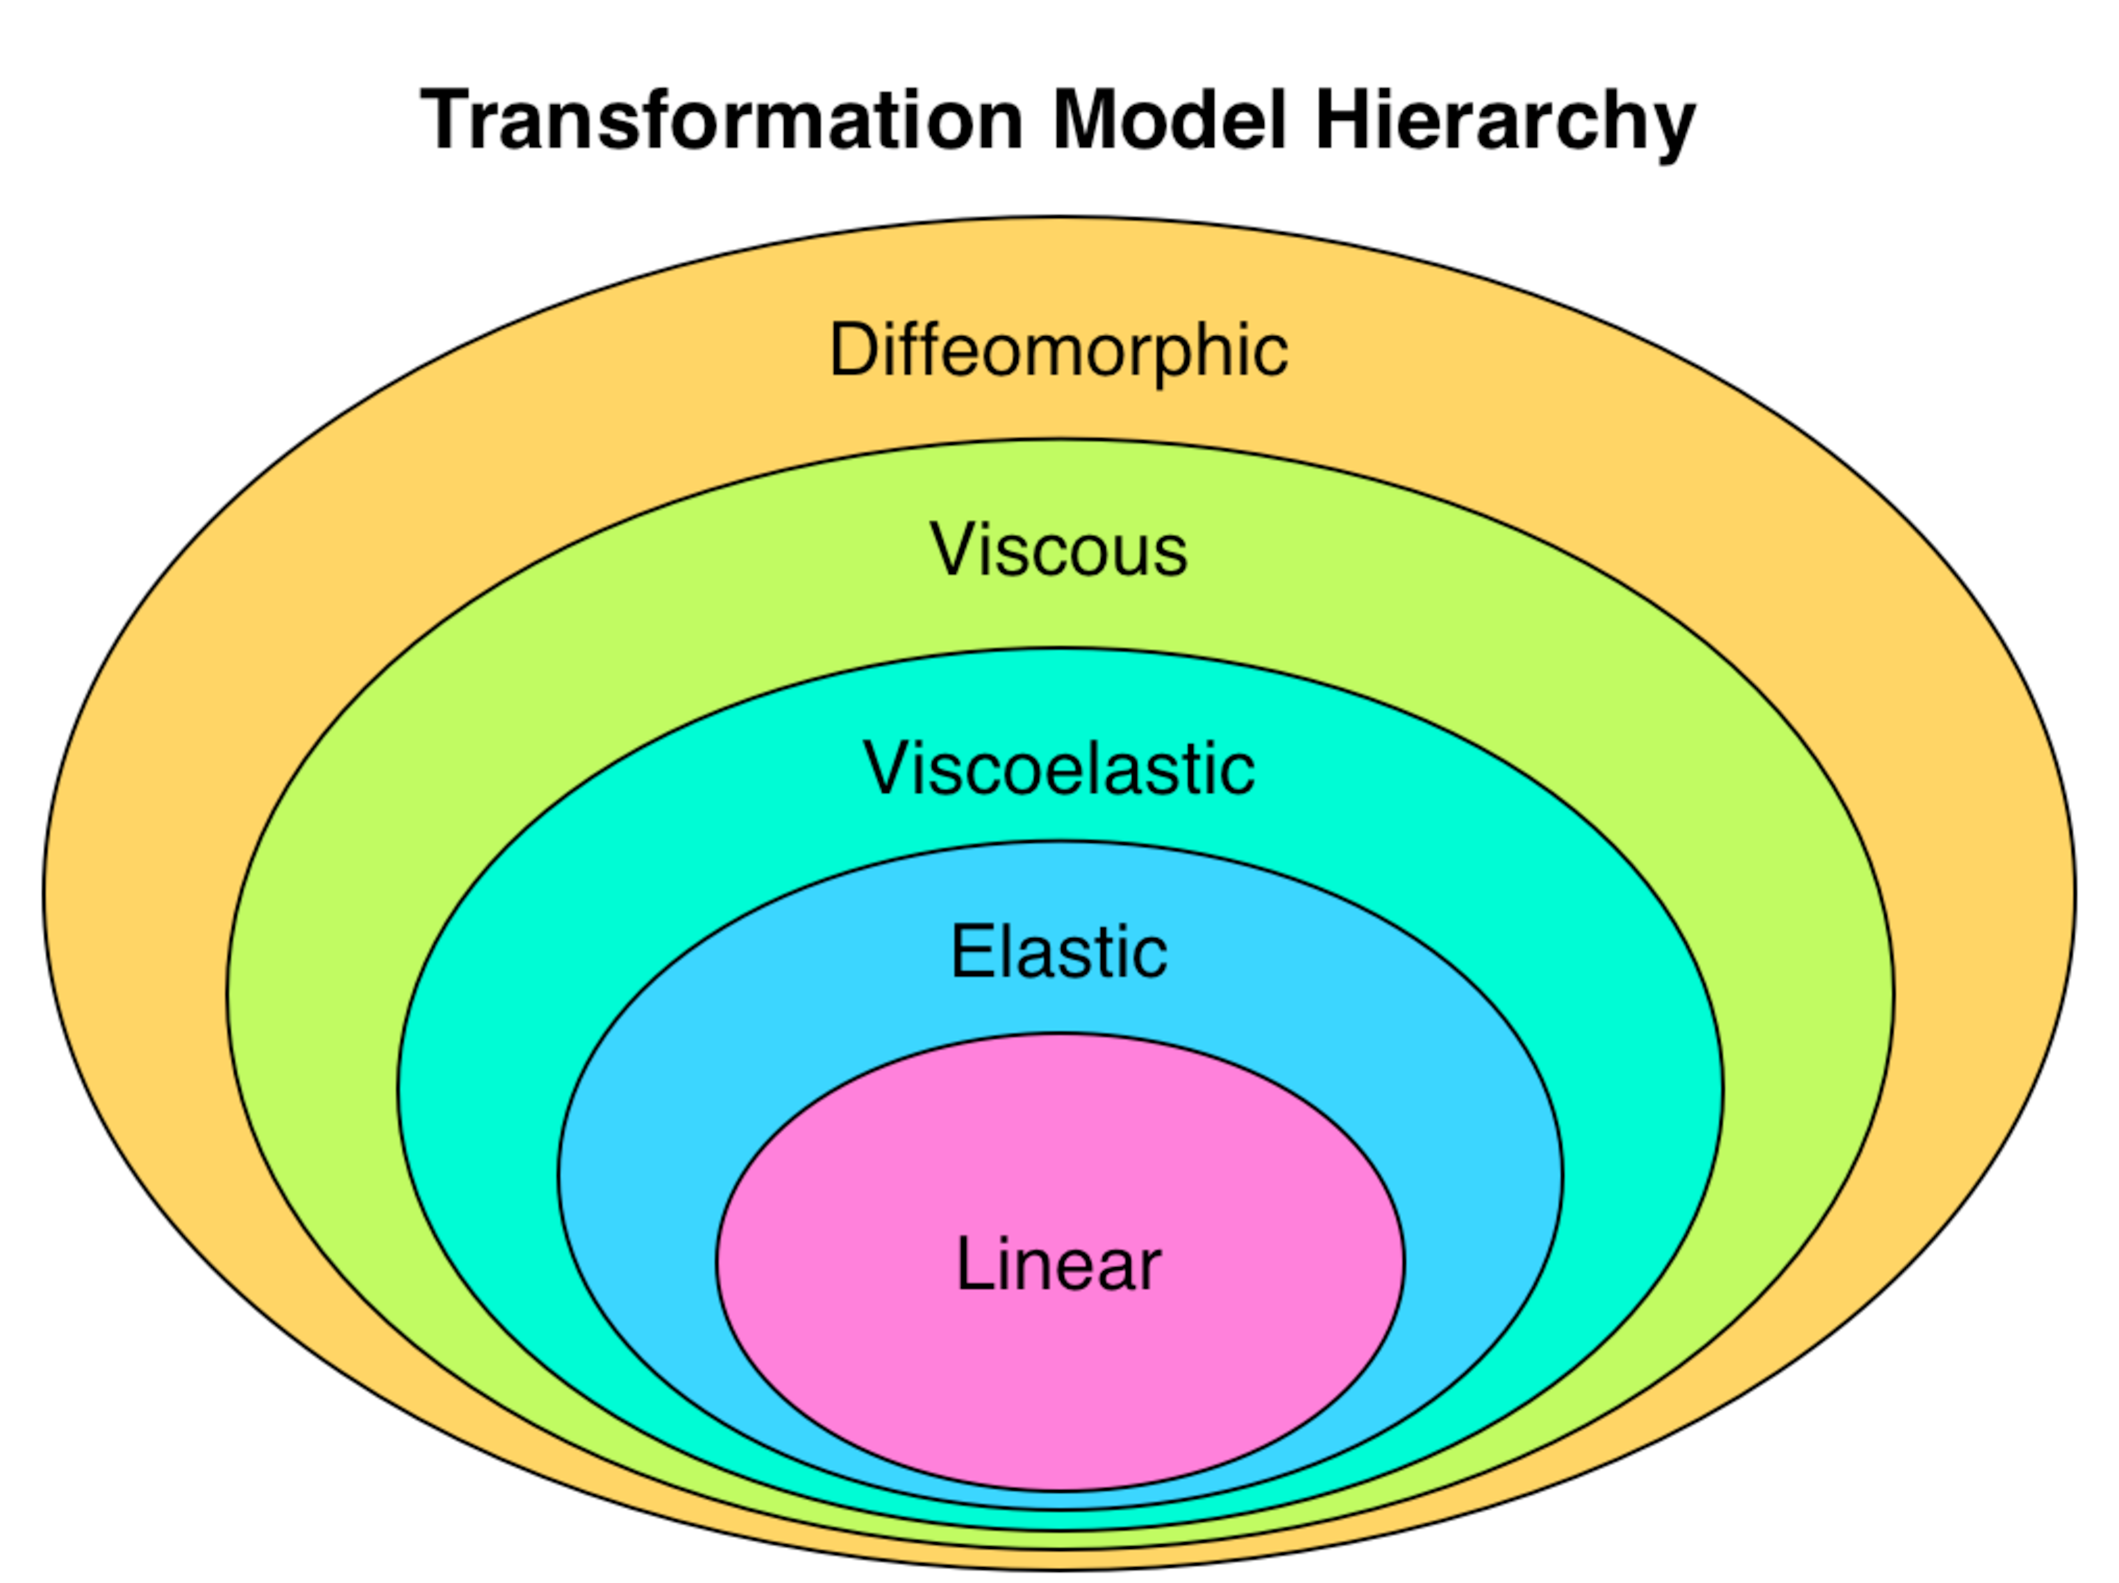
\includegraphics[width=80mm]{Figures/hierarchy}
    \end{tabular}
  \caption{Diagrammatic illustration of the transformation model hierarchy where the encompassing transformation spaces are characterized by increasing degrees of freedom.  }
  \label{fig:hierarchy}
\end{figure}
\subsubsection{Rigid and Affine Linear Transformations }
Image registration strategies often begin with a linear transformation
for initial global alignment which precedes a deformable
transformation with increased degrees of freedom.  The linear
transformations available within ANTS optimize either a mean-squared
difference (MSQ) or mutual information (MI) similarity metric which
are optimized with respect to translation, rotation, and, in the case
of affine transformations, scaling and shearing.  The successive
optimization of each component of the linear transformation allows for
careful control over increasing degrees of freedom.  ANTS also
composes the affine transformation with the deformable transformation
field before performing any interpolation or downsampling.  In this
way, ANTS normalization never requires more than a single image
interpolation step and is able to always refer back to the original
full-resolution image sources.  The ANTS implementation of rigid
mapping is quaternion-based with additional scaling and shearing terms
when affine mapping is desired (via the {\verb --rigid-affine } ~{\verb true } ~flag).  

\subsubsection{Vector Field Operators for Regularization} 
Deformable normalization strategies typically invoke a deformation
regularization step which smooths the displacement field, $\displace$,
or velocity field, $\mathbf{v}$, or both by a linear operator such as
the Laplacian or Navier-Stokes operator. One may write this
regularization as a variational minimization in terms of its linear
operator or in terms of a kernel function operating on the field
itself, e.g., $ \displace_{smooth}= K \star \displace_{not \,\,
  smooth}$, where $K \star$ denotes convolution with the Green's
kernel, $K$, for the linear operator, $L$.  Regularization models
operate on either the whole mapping $\phi$ or the gradient of the
similarity term or both.  The same regularization schema is available
for both diffeomorphic and the recently proposed directly manipulated
free-form deformation (DMFFD) \cite{Tustison2009}, allowing
regularization of both total deformation and deformation update.
Viewed from this perspective, hybrid configurations incorporating
discretized FFD strategies and diffeomorphisms can be combined for
novel image normalization approaches.  ANTS enables a variety of
choices for $K$ including the Gaussian with varying $\sigma$ and a
variety of B-spline functions, both of which induce adequate
regularity for normalization models used in ANTS.  While additional
physical operators will be included in future releases, current
B-spline options provide many orders of flexibility
\cite{Tustison2005}.

\subsubsection{Diffeomorphic Transformations}
Diffeomorphisms form a group of differentiable maps with
differentiable inverse \cite{Ebin1970,Mumford1998} that is closed
under composition.  In contrast, the vector space that most deformable
image registration methods use is closed under {\em addition}, an
operation that cannot guarantee topology preservation.  That is, two
topology-preserving vector fields added together are still a vector
field but the result may no longer preserve topology.  Furthermore,
most regularization models for vector spaces use a quadratic penalty,
thus making large deformations difficult to realize.  Modeling
transformations with diffeomorphisms, on the other hand, ensures a
flexible, linear penalty on deformation while guaranteeing topology
preservation.  Additionally, distance metrics in the space of
diffeomorphisms allow geodesic properties to be explored
\cite{Miller2001,Beg2005}.

ANTS assumes the diffeomorphism, $\phi$, is defined on the image
domain, $\Omega$, and maintains an affine transform at the boundary
such that $\phi(\partial \Omega) = A(\mathbf{Id})$ where
$A(\mathbf{Id})$ is an affine mapping applied to the identity
transformation.  The map $\phi$, over time, parameterizes a family of
diffeomorphisms, $\phi(\mathbf{x}, t) : \Omega \times t \rightarrow
\Omega$, which can be generated by integrating a (potentially) time-dependent,
smooth velocity field, $\boldsymbol{v} : \Omega \times t \rightarrow
\mathbb{R}^d$, through the ordinary differential equation (o.d.e.)
\begin{align} \label{eq:ode}
\frac{d \phi(\mathbf{x}, t)}{dt} = \boldsymbol{v}(\phi(\mathbf{x}, t),
t), \,\,\, \phi(\mathbf{x}, 0) = \mathbf{x}.
\end{align}
The existence and uniqueness theorem for o.d.e.'s implies that
integrating Equation (\ref{eq:ode}) generates a diffeomorphism.  The
deformation field yielded by $\phi$ is $\mathbf{u}(\mathbf{x}) =
\phi(\mathbf{x},1) - \mathbf{x}$.

Dupuis et al. \cite{Dupuis1998} motivated the usage of diffeomorphisms
for CA by showing that the variational form
\begin{align}\label{eq:D}
  D(\mathcal{I}, \mathcal{J}) = \int_0^1 ||L\boldsymbol{v}|| dt , \,\,
  \mathcal{I}(\phi(\mathbf{x}, 1)) = \mathcal{J}(\mathbf{z})
\end{align}
represents a true mathematical metric between anatomical instances
$\mathcal{I}$ and $\mathcal{J}$ given an appropriate norm, $L$, on the
velocity field, $\boldsymbol{v}$.  An optimal solution,
$\boldsymbol{v}^*$, minimizes the metric $D(\mathcal{I}, \mathcal{J})$
with respect to $L$.  Dupuis \cite{Dupuis1998} also showed that such a
solution is guaranteed to be well-posed.  Intuitively, Equation
(\ref{eq:D}) provides a sense of distance between two anatomical
shapes.  It also illustrates that the optimal diffeomorphic solution
is analogous to finding the geodesic curve between two points in a
curved space.
\footnote{ It is important to note the similarity between the
  definition of curve length, $\int ||\mathcal{C}'(t)||dt$, for the
  parametric curve $\mathcal{C}(t)$ and Equation (\ref{eq:D}).  In
  this sense, the solution for Equation (\ref{eq:D}) is the geodesic
  diffeomorphism, where $\boldsymbol{v}$ is the tangent vector of the
  diffeomorphism, such that the shape distance, $D$, between
  $\mathcal{I}$ and $\mathcal{J}$ is minimized.  }

In most real-world applications, however, a diffeomorphic path
connecting the anatomical instance $\mathcal{J}$ with $\mathcal{I}$ is
non-existent (due, for example, to photometric variation, idiosyncratic cortical folding or the
presence/absence of a tumor in neuroanatomical images).  Therefore,
the following minimizing variational form is used for optimization in
diffeomorphic normalization to accommodate inexact matching
\cite{Dupuis1998,Miller2002}
\begin{align} \label{eq:lddmm}
  \boldsymbol{v}^* = \underset{\boldsymbol{v}}{\operatorname{argmin}}
  \left\{ \int_0^1 ||L\boldsymbol{v}||^2dt + \lambda\int_{\Omega} ||
  \mathcal{I} \circ \phi(\mathbf{x},1) - \mathcal{J} || d\Omega
  \right\}.
\end{align}
The Euler-Lagrange equations characterizing the optimizing
time-varying velocity field, $\boldsymbol{v}^*$, were derived in
\cite{Miller2002} and later used in formulating the gradient-descent
optimization scheme known as {\em large deformation diffeomorphic
  metric-matching} (LDDMM) \cite{Beg2005} with the similarity metric,
or data term, for LDDMM being the squared intensity difference with
weight $\lambda$.

To accommodate a variety of medical image normalization tasks, one
typically encounters more complex intensity transfers between one
anatomical instance $\mathcal{J}$ and another instance $\mathcal{I}$.
Thus, ANTS enables not only a variety of similarity metric
possibilities beyond the conventional squared difference metric but it
also permits any number of different similarity metrics for a
particular image normalization task.  This leads to the following
generalization of Equation (\ref{eq:lddmm}):
\begin{align} \label{eq:diff}
  \boldsymbol{v}^* = \underset{\boldsymbol{v}}{\operatorname{argmin}}
  \left\{ \int_0^1 ||L\boldsymbol{v}||^2 dt
  +\lambda\int_{\Omega}\Pi_{\sim}( \mathcal{I}, \phi(\mathbf{x},1) ,
  \mathcal{J} )d\Omega \right\}
\end{align}
where $\Pi_{\sim}$ is a similarity metric depending on the images and
the mapping and $\lambda$ controls the degree of exactness in the
matching.  If $\Pi_{\sim}$ is selected as cross-correlation, then one
is estimating the diffeomorphism under more robust illumination
constraints, as described in \cite{Avants2008}.  

Exploiting the fact that the diffeomorphism, $\phi$, can be decomposed
into two components $\phi_1$ and $\phi_2$, one may construct a {\em
  symmetric} alternative to Equation (\ref{eq:diff}).  Now define, in
$t \in [0,0.5]$, $\boldsymbol{v}(x,t) = \boldsymbol{v}_1(x,t) $ and
$\boldsymbol{v}(x,t) = \boldsymbol{v}_2(x,1-t)$ when $t \in [0.5,1]$.
This leads to the symmetric variant of Equation (\ref{eq:diff}),
\begin{align}\label{eq:diffs}
  \{ \boldsymbol{v}^{*}_1 , \boldsymbol{v}^{*}_2 \}= &
  \underset{\boldsymbol{v}_{1,2}}{\operatorname{argmin}} \Bigg\{
  \nonumber \\ & \int_0^{0.5} ||L\boldsymbol{v}_1(x,t)||^2 ~dt +
  \int_0^{0.5} ||L\boldsymbol{v}_2(x,t)||^2 ~dt \nonumber \\ &+
  \lambda\int_{\Omega}\Pi_{\sim}\left( \mathcal{I} \circ
  \phi_1(\mathbf{x},0.5), \mathcal{J}\circ
  \phi_2(\mathbf{x},0.5)\right)d\Omega\Bigg\}.
\end{align}
Note that the regularization term, here, is equivalent to that in
equation~\ref{eq:lddmm}.  The only change is the splitting of the
integral into two time intervals reflecting the underlying optimized
components of the velocity field.  The corresponding symmetric
Euler-Lagrange equations are similar to \cite{Miller2002}.  The
difference, here, is that in finding $\boldsymbol{v}^*$, we minimize
the variational energy from either end-point towards the mid-point of
the transformation, as indicated by the data term.  This strategy
``splits'' the optimization dependence equally between both images.
Thus, gradient-based iterative convergence deforms $\mathcal{I}$ and
$\mathcal{J}$ along the geodesic diffeomorphism, $\phi$, to a fixed
point midway (intuited by the notion of shape distance) between
$\mathcal{I}$ and $\mathcal{J}$ thus motivating the denotation of the
solution strategy as Symmetric Normalization (SyN).

Other diffeomorphic algorithms have since been reported in the
research literature e.g. DARTEL \cite{Ashburner2007} and Diffeomorphic
Demons \cite{Vercauteren2007,Vercauteren2009}, both of which use the
constant velocity, exponential model for generating diffeomorphisms.
We thus include three diffeomorphic transformation models for
parameterizing $\phi(\cdot)$.  These include Geodesic SyN, Greedy SyN,
and exponential mapping.  As summarized in Table \ref{table:chart},
each of these transformation models can utilize a host of similarity
measures both individually and in mutual combination.

%Briefly, ANTS diffeomorphic transformation models are: 
%\begin{enumerate}
%\item {\bf Exponential Mapping:}  This constant velocity field parameterization does not produce a distance metric; maps are not dense in the space of diffeomorphisms and are not inverse consistent.
%\item {\bf Greedy SyN:} Approximates the distance metric with a fast approach.  Evaluated in \cite{Klein2009}.  Enforces $\phiinv(\phi(\x,1))=\x$ in the discrete domain.  Theoretically and computationally inverse consistent / symmetric. 
%\item {\bf Geodesic SyN:}  Symmetrically minimizes the velocity field / distance metric explicitly over all time.  Computationally more expensive than, but produces similar solutions to, Greedy SyN for most medical imaging problems.
%\end{enumerate}
%All of these transformation models may be used with any of the ANTS similarity metrics.  In particular, ANTS allows $\Pi$ 
%to be composed of a summation/weighted combination of available similarity metrics/data terms.

\paragraph{Geodesic SyN}
Using a gradient-based optimization strategy for minimizing equation
(\ref{eq:diffs}) first requires a specified discretization of $t$,
s.t. $t \in [0,1] \approx \{ 0 , 1/k , 2/k , \cdots , 1 \} $ where
integer $k > 1$ is the desired number of discretized intervals.
Calculation of the gradient of $\Pi$ with respect to the
diffeomorphisms $\phi_1$ and $\phi_2$ is performed at each of these
$t$ values, $t_k$,
\begin{align}
\label{eq:grad}
  \nabla \Pi_i(\boldsymbol{x},t_k) = \frac{\partial}{\partial \phi_i}
  \Pi_{\sim}( \mathcal{I}(\phi_{1}^{-1}(\boldsymbol{x},t_k)),
  \mathcal{J}(\phi_{2}^{-1}(\boldsymbol{x},1-t_k))
\end{align}
for $i \in \{1,2\}$.  The total velocity field is then updated from
the previous iteration according to, for each $i$,
\begin{align}
  \boldsymbol{v}(\mathbf{x},t) = \boldsymbol{v}(\mathbf{x},t) + \delta
  K \star \nabla \Pi_i(\mathbf{x},t),
\end{align}
where $\delta$ is the user-specified gradient descent parameter.  Note
that the update, here, is a $N+1$-dimensional vector field and $K$ is
a $N+1$-dimensional operator, when the images are $N$ dimensions.  We
generate $\phi_i(\mathbf{x},t)$ for each $t \in [0,1]$ and $i \in
\{1,2\}$ by integrating Equation (\ref{eq:ode}) using Runge-Kutta methods.  
We cycle through these steps until convergence or iterative exhaustion.

\paragraph{Greedy SyN}
Although the Geodesic SyN algorithm conforms most closely to the
theoretical diffeomorphic foundations culminating with Equation
(\ref{eq:diffs}), the computational and memory cost is significant due
to the dense-in-time gradient calculations and requisite reintegration
of the diffeomorphisms after each iterative update.  As a lower-cost
alternative, we offer a greedy variant which performs quite well for
most medical image normalization problems we have encountered.
Additionally, this was the strategy used in the large-scale
comparative image registration algorithm assessment of
\cite{Klein2009}.

Greedy optimization of Equation (\ref{eq:diffs}) calculates the
gradient only at the mid-point of the full diffeomorphism, i.e. at $t
= 0.5$ in equation~\ref{eq:grad}
\begin{align} 
\nabla \Pi =\frac{\partial}{\partial \phi_i} \Pi_{\sim}(
\mathcal{I}(\phiinv_1(\x,0.5)) , \mathcal{J}(\phiinv_2(\x,0.5)) )
\end{align} 
for $i \in \{1,2\}$.  $\phi_1(\mathbf{x},0.5)$ and
$\phi_2(\mathbf{x},0.5)$ are then updated from the previous iteration
according to
\begin{align}
  \phi_i(\mathbf{x},0.5) = \phi_i(\mathbf{x},0.5)+ (\delta K \star
  \nabla \Pi_i(\mathbf{x},0.5) ) \circ \phi_i(\x,0.5).
\end{align}
That is, the gradient at the mid-point is mapped back to the origin of
each diffeomorphism.  We then update the full mapping by explicitly
enforcing $\phiinv(\phi(\x,1))=\x$ in the discrete domain, as
described in \cite{Avants2008}.

\paragraph{Exponential Mapping}
Ashburner introduced DARTEL (Diffeomorphic Anatomical Registration
using Exponentiated Lie algebra) as a rapidly computed alternative to
time parameterized diffeomorphic schemes \cite{Ashburner2007}.  The
key difference between a time-varying diffeomorphism and a
diffeomorphism generated by an exponential mapping
\cite{Ashburner2007} is that the exponential mapping maintains only a
single vector field that is constant in time.  A diffeomorphism can be
generated by exponentiation of a constant velocity field from the
following o.d.e (cf Equation (\ref{eq:ode}))
\begin{align} \label{eq:odec}
\frac{d \phi(\mathbf{x}, t)}{dt} = \boldsymbol{v}(\phi(\mathbf{x},t)
), \,\,\, \phi(\mathbf{x}, 0) = \mathbf{x}.
\end{align}
Note that there is no explicit time parameter in the velocity field.
Theoretically, restricting the velocity field to be constant in time
reduces the size of the space that may be generated \cite{Arnold1991}
in a way that is similar to the difference between real and rational
numbers, the latter of which are sparsely distributed through the
reals.  ANTS registration via exponential mapping optimizes the functional,
\begin{align}\label{eq:diffexp}
    \nonumber \\ & ||L\boldsymbol{v}(x)||^2 +
    \lambda\int_{\Omega}\Pi_{\sim}\left( \mathcal{I} ,
    \mathcal{J}\circ \phi(\mathbf{x},1)\right)d\Omega.
\end{align}
ANTS currently updates the velocity field based on the gradient only
at the end-point.  That is, the gradient is computed after the image
$\mathcal{J}$ is mapped to the ``fixed'' image $\mathcal{I}$.  In
contrast, DARTEL optimizes over the time discretization, computing the
gradient at each discrete time point, as in the full ANTS geodesic optimization. 
However, ANTS also allows a greedy exponential mapping strategy 
that is analogous to the method described in \cite{Vercauteren2009} (\verb GreedyExp ). 
An important difference between Diffeomorphic Demons and exponential mapping 
is that Diffeomorphic Demons composes exponential maps together.  It is therefore 
closer to a greedy descent strategy similar to that used in Christensen's classic approach \cite{Christensen96}.

\subsubsection{Vector Space Transformations}
Potential mapping solutions to the image matching problem operating in
vector spaces are constructed in a similar variational form as that
for the diffeomorphic formulation.  We write this general variational
energy, $\Pi$, as
\begin{align} \label{eq:energy}
  \Pi(\mathcal{I}, \mathcal{J}, \phi) = \int_{\Omega}
  \left(\Pi_{\sim}(\mathcal{I}, \mathcal{J}, \phi)(\mathbf{x}) +
  \lambda~ \Pi_{R}(\phi)(\mathbf{x})\right) d\Omega,
\end{align}
where $\mathcal{I}$ and $\mathcal{J}$ are, again, the moving and fixed
images, respectively, and $\phi$ is the transformation which maps
between $\mathcal{I}$ and $\mathcal{J}$.  $\Pi_{\sim}$ is the
similarity metric and $\Pi_{R}$ is the explicit regularization term.

\paragraph{Gaussian-Regularized Elastic Deformation}
A simple and efficient, yet powerful image normalization algorithm is
the approach known as Thirion's demons \cite{Thirion1998}.  Using an
optical flow based similarity, the solution is obtained by iterating
between the calculation of image forces and subsequent Gaussian
regularization.  In ANTS, we extend this basic approach to include the
similarity metrics available for deformable registration (see Table
\ref{table:chart}).  This leads to an update form that is performed 
as follows: 
\begin{eqnarray} 
{\bf U}=\frac{\partial}{\partial \phi} \Pi_{\sim}(\mathcal{I}(\x), \mathcal{J}(\phiinv(\x))), \notag \\ 
\mathbf{u}(\mathbf{x}) = K_{\mathbf{u}} \star ( \mathbf{u}(\mathbf{x}) + \delta  K_{\bf U} \star {\bf U}), 
\end{eqnarray}
where $K_{\mathbf{u}}$ regularizes the total deformation field and 
$ K_{\bf U} $ regularizes the gradient field.   \footnote{
Any ANTS transformation model may be used with both 
update and total deformation regularization.}
Thus, ANTS vector field transformation models default to a 
Demons style optimization.  Like the Demons algorithm, this 
method uses a greedy descent on the energy and does not 
truly optimize the total variational form.  The update strategy 
for the exponential mapping is very similar to the above, but 
with an additional composition on the gradient that maps the gradient 
back to time zero.  See \cite{Vercauteren2009} for a nice discussion 
of the distinction between additive and compositive updates in these methods. 



\subsection{ANTS Intensity-Based Similarity Metrics}
Several intensity-based image metrics have been proposed in the
literature with varying levels of performance dependent upon specific
applications.  We have included several of the most popular similarity
metrics within ANTS.  In addition, our software framework facilitates
the development of other image metrics.  Both mutual information
\cite{Viola1997} and mean-squared difference similarity metrics are
available for the linear transformations.  Also included are the
cross-correlation (the PR metric) \cite{Avants2007b}, local mutual
information \cite{Rueckert1999,Pluim2003}, and mean squared difference
similarity metrics for the non-linear transformation models.  The
parameters for the different metrics are discussed in the ANTS
documentation \cite{ANTS2009}.  The cross-correlation uses a local
neighborhood in a spatially varying correspondence model which
provides robustness to illumination and inhomogeneity.  Therefore, we
choose the correlation metric for most practical image registration
problems in real imagery.
  
\subsection{ANTS Label or Point-Based Similarity Metrics}
In addition to intensity-based metrics, ANTS also contains similarity
metrics for registering labeled point-sets or label images.  These
include a landmark matching metric and two point-set metrics which can
accommodate point-sets of different cardinality.  These point-set
metrics can be used alone for strict point-set registration or in
conjunction with intensity-based metrics for dual intensity/point-set
registration.  Exact matching and partial (or incompletely labeled)
point set matching are available.


\subsubsection{Exact Landmark Matching}
Generalizing the B-spline fitting algorithm of \cite{Lee1997}, we
developed a scattered data approximation algorithm
\cite{Tustison2006b} and contributed the code to the ITK library
\cite{Tustison2005}.  This code is included in ANTS and forms the
basis of our exact landmark matching where this metric seeks to
minimize the weighted sum of distances between corresponding landmarks
using a hierarchical approach.  One can also associate relative
confidence values with each landmark for fine-tuning exact landmark
matching results.


\subsubsection{Point-Set Expectation}
In \cite{Pluta2009}, the point-set matching problem was formulated in
the context of incomplete label matching but is equally applicable to
the general scenario of registering point-sets not necessarily of
equivalent cardinality.  Given two point-sets, $X$ and $Y$, the
essential idea underlying the point-set expectation matching algorithm
is that the optimal solution minimizes the distance between each point
$y \in Y$ with its corresponding {\em expected} point in $X$.  
When discussing these point-based metrics, we abuse notation 
slightly by ``hiding'' the application of the deformation to the points to 
simplify the notation.  However, in practice, we apply the same mapping 
to the points as we do to the imagery that is associated with them and that 
defines their spatial domains.  Thus, the transformations that appear 
in the image similarity term are also used in the point similarity for all below. 

We calculate the expected point using a Bayesian formulation and a
non-parametric Parzen windowing scheme.  This allows one to define the
probability of the point $x \in X$ given a point $y\in Y$ as
\begin{align}
  \mathbf{P}(X = x | Y = y ) = G(y; x, \sigma_X )
\end{align}
where $G(y; x, \sigma_X)$ is a normalized Gaussian with mean $x$ and
standard deviation $\sigma_X$.  The expected point $\mathrm{E}(X|y)$
is then calculated to be
\begin{align} \label{eq:expected}
  \mathrm{E}(X | Y = y) &= \sum_{j = 1}^{|X|} \mathbf{P}(X = x_j | Y =
  y ) x_j\nonumber \\ &= \frac{1}{|X|}\sum_{j = 1}^{|X|} G(y; x_j,
  \sigma_X) x_j
\end{align}
where $|\cdot|$ denotes cardinality.  The weighted sum of distances
between the points in $Y$ and their corresponding expected points in
$X$ is calculated from Equation (\ref{eq:expected}), i.e.
\begin{align}
\mathrm{PSE}(X,Y) = \frac{1 }{|Y|}\sum_{i=1}^{|Y|} \left\|y_i -
\frac{1}{|X|} \sum_{j = 1}^{|X|} G(y_i; x_j, \sigma_X) x_j\right\|^2.
\end{align}
The ANTS parameters for this metric require one to choose the percentage of points to use 
from the input data (subset selection increases efficiency), the Parzen window sigma ($\sigma_X$), 
the number $K$ for the number of nearest neighbors used in the Parzen window calculation (again for efficiency) 
and, finally, the number of iterations over which one optimizes the similarity symmetrically.  
This latter option is useful for partial matching problems as in \cite{Pluta2009}. 
A related similarity metric, based on maximizing the Jensen-Havrda-Charvat-Tsallis Divergence 
between the point sets, is described in the appendix. 

\section{ANTS Implementation and Usage}
\label{sec:imp}
ANTS, built upon an ITK foundation, maintains the same coding style as its base.  For much of its functionality, ANTS requires ITK, necessitating the installation of ITK prior to installing ANTS.  All ANTS source code is available via the online source code repository SourceForge.%
\footnote{
http://sourceforge.net/projects/advants/
}
Binaries for Windows, OSX, 32 and 64-bit Linux are also available from the same online location.  For quality assurance and maintenance purposes we have established an ANTS test reporting open-source ``dashboard''%
\footnote{
http://www.cdash.org
}
 on our lab website%
\footnote{
http://www.picsl.upenn.edu/cdash/index.php?project=ANTS
}
to monitor compilation and testing of the ANTS program.  A screenshot from a daily testing period is given in Figure \ref{fig:dashboard}.  Such a configuration facilitates reporting of problems encountered by users on a multitude of computing platforms.   

\begin{figure*}
\centering
  \begin{tabular}{c}
      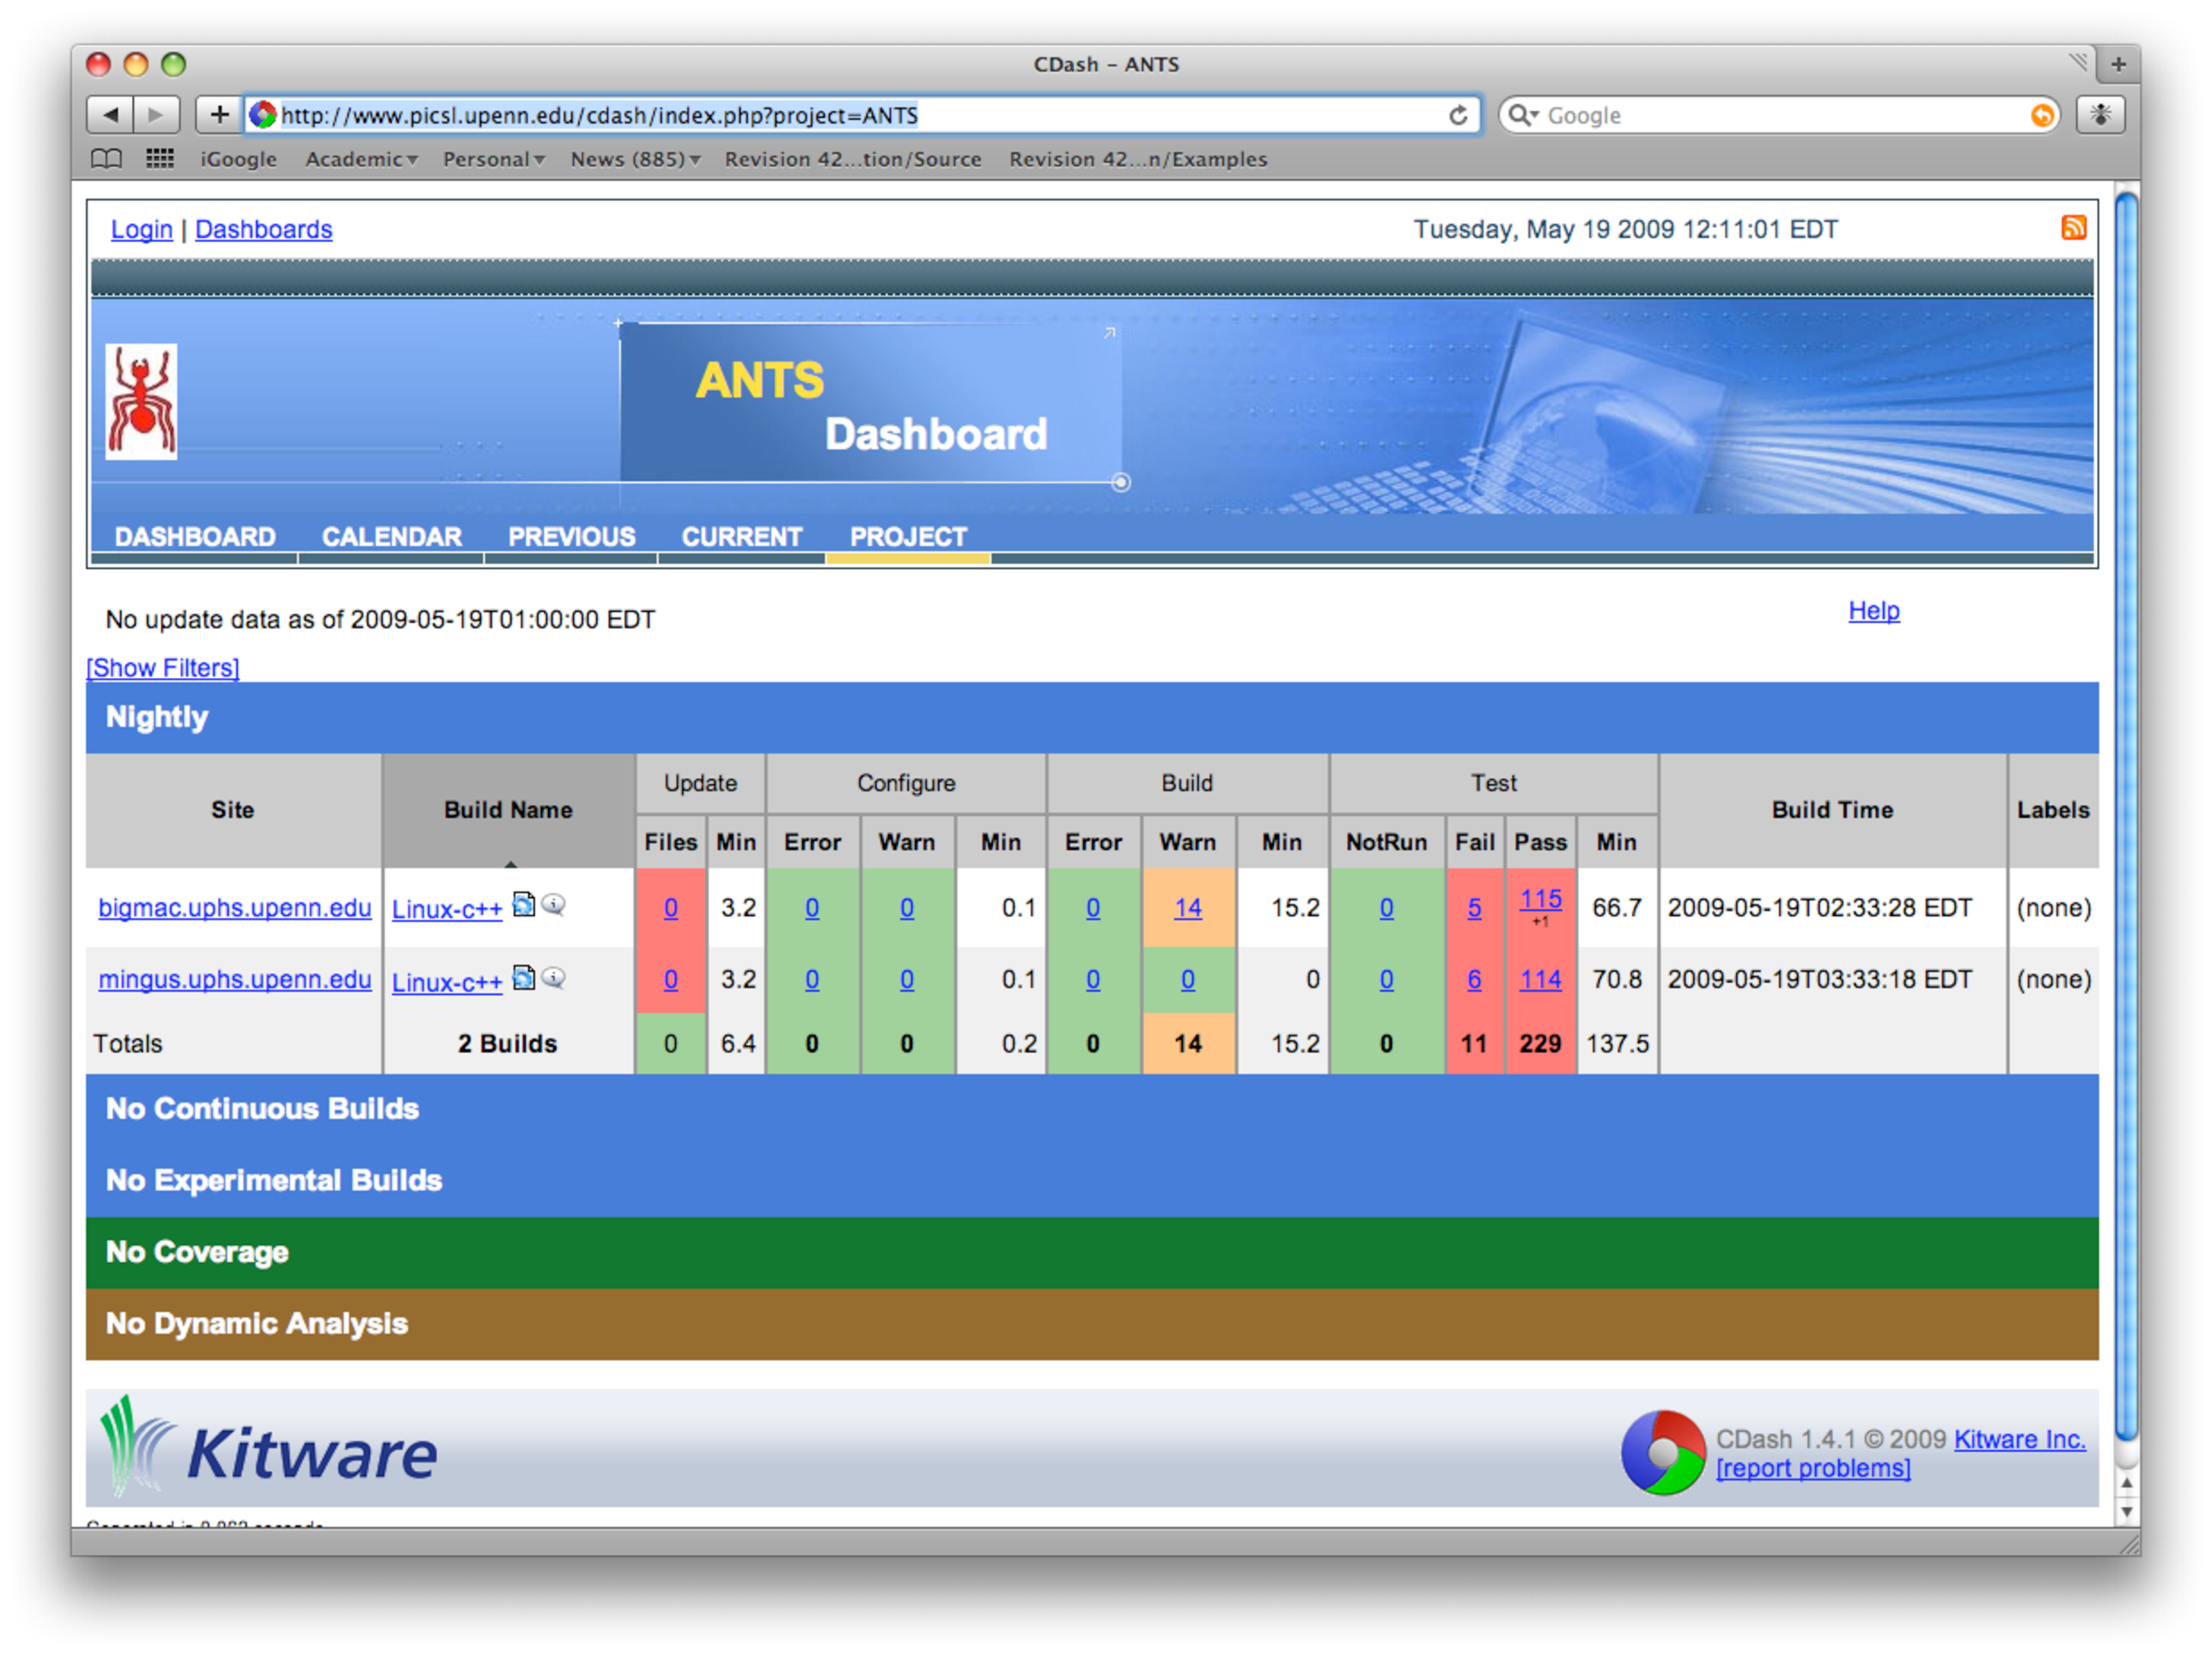
\includegraphics[width=135mm]{Figures/ANTSdashboard} 
  \end{tabular}
\caption{The ANTS dashboard, which is hosted on the PICSL website, reports daily building and testing of the ANTS software.  It also allows any user to submit their own building and testing configurations to help with debugging issues and maintenance for a variety of computing platforms. }  
\label{fig:dashboard}
\end{figure*}


% ADD_TEST(ANTS_PSE_MSQ_IMG ANTS 2 -i 191x170x90x90x10  -r Gauss[6,0.25] -t SyN[1,2,0.1] 
%                             -m PSE[${DEVIL_IMAGE},${ANGEL_IMAGE},${DEVIL_IMAGE},${ANGEL_IMAGE},0.25,0.1,100,0,10]
%                             -m MSQ[${DEVIL_IMAGE},${ANGEL_IMAGE},1,0.1]
%                              --continue-affine 0 --number-of-affine-iterations 0 --geodesic 2 
%                             -o ${OUTPUT_PREFIX}.nii)

Based on our experience with standard command line argument parsing packages (e.g. \verb#getopt#), we developed our own set of classes for an intuitive command line interface.  A summary of command line arguments are given in Table \ref{table:args}.  
These ANTS argument parsing classes provide an intuitive compromise between parsers where every variable requires a unique flag and strict ordering requirements on the command line.  A multivariate command line call to ANTS  is  given by:
\begin{lstlisting}
>ANTS 3 
  --metric MSQ[fixedImage.nii,movingImage.nii,1] 
  --metric PSE[fixedImage.nii,movingImage.nii,
     fixedLabels.nii,movingLabels.nii,0.25,0.1,100,0,10] 
  --transformation SyN[1,2,0.1] --geodesic 2  
  --regularization Gauss[6.0,0.25]
  --iterations 50x20x10x5 
  --output-naming results.nii
\end{lstlisting}
The MSQ metric uses weight 1 while the PSE metric has weight 0.25.  In
the PSE metric, ten percent of points are selected from the Label
images (param 0.1).  The point set variance is 100, points are
selected densely (not just from the boundaries of the labels) and 10
nearest neighbors are used.  The transformation model is the full time
optimization of the symmetric SyN transformation (chosen by including 
 --geodesic 2) with gradient step 1, two
time points in the spatiotemporal discretization and a time-step of
0.1 in the Runge-Kutta integration that generates the diffeomorphisms.
The correspondence between the ANTS command line specification and the
image normalization formulation with images $I$ and $J$ and their corresponding labeled images $X$ and $Y$ 
illustrates the motivation for our command line interface,
\begin{align}
  \Pi(\mathcal{I},\mathcal{J},X,Y,\phi)
     = \underbrace{\int_0^1 ||L\boldsymbol{v}(x,t)||^2 dt}_{\texttt{-t SyN[}\cdot \texttt{]},\texttt{ -r Gauss[}\cdot\texttt{,}\cdot\texttt{]}}  +  \nonumber \\ 
 \underbrace{\lambda_1\int_{\Omega} || \mathcal{I} \circ \phi_1(\mathbf{x},0.5) - \mathcal{J}\circ \phi_2(\mathbf{x},0.5)  || d\Omega}_{\texttt{ -m MSQ[}\mathcal{J}\texttt{,}\mathcal{I}\texttt{,}\lambda_1\texttt{]}} \nonumber \nonumber + \\
\underbrace{\frac{\lambda_2 }{|Y|}\sum_{i=1}^{|Y|} \left\|y_i - \frac{1}{|X|} \sum_{j = 1}^{|X|} G(y_i; x_j, \sigma_X) x_j\right\|^2}_{\texttt{-m PSE[}Y\texttt{,}X\texttt{,}\lambda_2\texttt{]}}.
\end{align}
Here, we apply the expectation-based point set registration method 
for mapping labeled points sets, as described in \cite{Pluta2009}.   ITK-SNAP may be used to label 
images and exported segmentation images may be input to the 
PSE metric below, as labeled data.  The Frown and Smile data is used 
as example and is shown in figure~\ref{fig:frown}.  This data is available in the 
ANTS/Examples/Data/ directory.
\begin{figure}
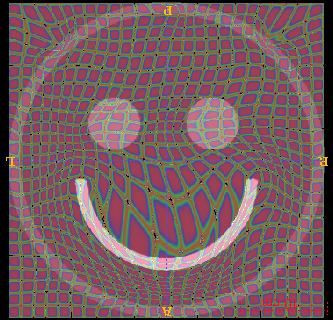
\includegraphics[width=0.45\textwidth]{Figures/frowntosmile.png}
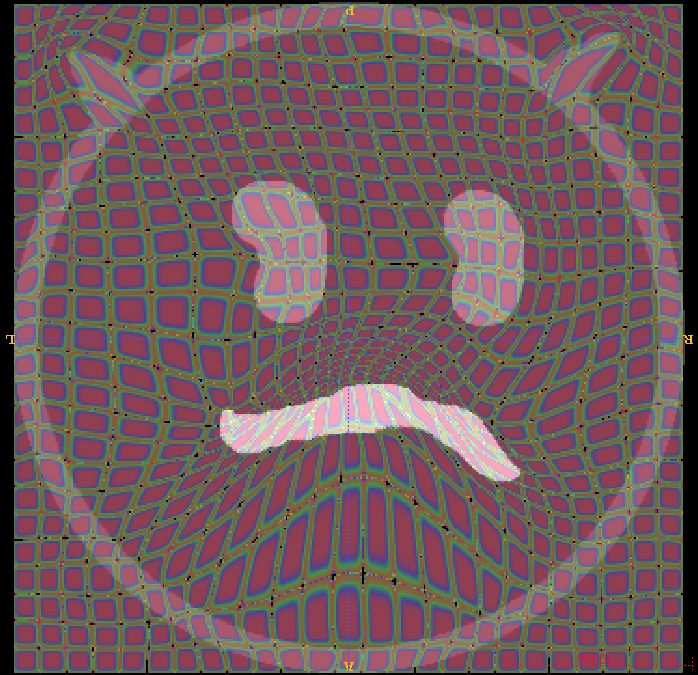
\includegraphics[width=0.45\textwidth]{Figures/smiletofrown.png}
\caption{Expected output for the frown to smile 
shows a smooth, though large deformation.  The grids are overlaid on 
the deformed images.  In this case, the label images and the similarity metric images are identical.  
The labelings are important for guiding this image mapping to a good local minimum.  Without the 
label guidance, an accurate mapping between the ``smile'' and the ``frown'' cannot be achieved 
as the image similarity term only maps part of the image correctly.  Users may run the example 
themselves as all data is available in the ANTS toolkit Examples/Data directory.  
\label{fig:frown}}
\end{figure}
This example should run on the downloaded ANTS data so you may see the
results.  The ANTS CMakeLists.txt file contains the command that runs
this data in automated testing (via the CMake ctest command) and
allows the user to evaluate whether s/he is getting the expected
performance from their own installation.  In Table \ref{table:args} we
give a brief summary of the arguments available for the normalizations
offered by the ANTS package.  This includes the corresponding variable
specification.  More information can be found on the ANTS website.

\begin{table*}
  \centering
    \begin{tabular}{c c c c c}
   {\bf } & {\bf Argument} & {\bf Flag} & {\bf Variables}  & {\bf Sample Parameters}\\
    \toprule
    \multirow{3}*{\bf Linear}
    & Iterations & \verb#--linear-iterations# & {} & $N_1$\verb#x#$N_2$\verb#x#$N_3$\verb#x#\ldots \\ 
    & Similarity & \verb#--linear-metric# & \verb#MI,MSQ# & \verb#[#$N_{bins}$,$N_{samples}$\verb#]# \\ 
    {} & Affine or Rigid &  \verb#--do-rigid# & {} & \verb#true / false # \\
    \cmidrule(l){2-5}
    \multirow{5}*{\bf Deform.}
    & Image Similarity & \verb#--metric,-m# & \verb#MI,CC,PR,MSQ# & \verb#[#$\mathcal{I},\mathcal{J}$,\verb#radius]# \\
    & Point-Set Similarity & \verb#--metric,-m# & \verb#PSE,JHCT# & \verb#[#$\mathcal{I},\mathcal{J},X,Y$\verb#]# \\
    {} & Iterations/Level & \verb#--iterations,-i# & {} & $N_1$\verb#x#$N_2$\verb#x#$N_3$\verb#x#\ldots \\ 
    {} & Regularization &  \verb#--regularization,-r# & \verb#Gauss,DMFFD# & \verb#[#$\sigma^2_{gradient}$,$\sigma^2_{total}$\verb#]#, \verb#[1x1,3x3]#\\
    {} & Transformation & \verb#--transformation,-t# & \verb#Elast,SyN,Exp# & \verb#[#$\Delta_{gradient}$\verb#]# \\   
    {} & Transformation & \verb#--large-deformation# & \verb#SyN# & \verb#[#$\Delta_{gradient}$,\# time points,dT\verb#]# \\
    \cmidrule(l){2-5}
    \multirow{2}*{\bf Misc.}
    & Histogram Match $\mathcal{I},\mathcal{J}$ & \verb#--use-histogram-matching# & {}  & \verb#1# \\
    {} & NN Interpolation & \verb#--use-NN# & {} & \verb#0#\\
    {} & Mask Image &  \verb#--mask,-x# & {} & \verb#mask.nii# \\
    {} & Output Naming     & \verb#--output-naming,-o# & {} & \verb#filename.nii# \\
    \bottomrule
    \end{tabular}
  \caption{The various flags and variables for a variety of image registration possibilities.   Additional information can be found on the ANTS website \cite{ANTS2009}. }
  \label{table:args}
\end{table*}    

\section{Experimental Evaluation}
\label{sec:expt}
The first part of our experimental evaluation will assess ANTS
performance on qualitative, ``classic'' examples of large deformation
image registration.  Two examples will suffice, both of which are
based on the letter ``{\bf C}'' examples pioneered by
\cite{Christensen96} and also used in \cite{Vercauteren2009}.  The
purpose of these examples is to show large deformation capabilities
with different transformation options.  We follow this example with
experiments that assess whether, in the cortical labeling problem with
normal control data, the added flexibility of true large deformation
implementations conveys a performance advantage.

\subsection{Classic Registration Examples}
The classic C examples are used to illustrate differences in the
ability of image registration transformation models to achieve
``large-deformation'' mappings between images.  While good performance
in these examples provides little insight about normalization of real
brain imagery, one is able to evaluate the relative accuracy and
flexibility of the transformation model when topology and similarity
concerns are minimized.  An example is shown in
figure~\ref{fig:chalf}.
\begin{figure}
\begin{center}
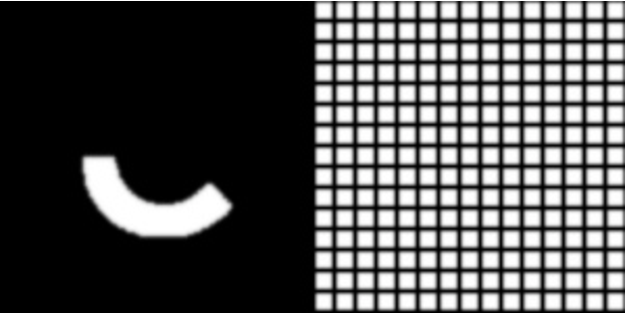
\includegraphics[width=0.33\textwidth]{Figures/grid1100.pdf}
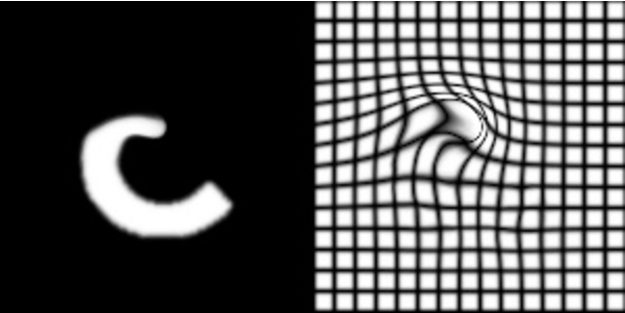
\includegraphics[width=0.33\textwidth]{Figures/grid1110.pdf}
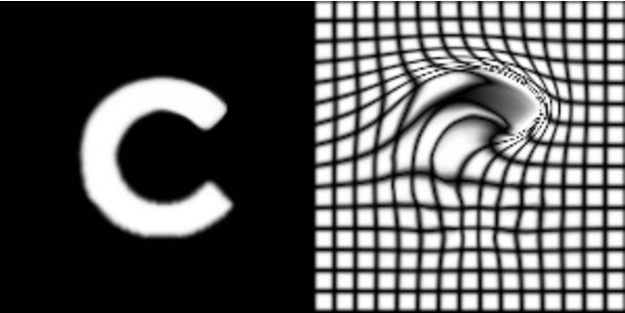
\includegraphics[width=0.33\textwidth]{Figures/grid1119.pdf}
\end{center}
\caption{ANTS Large Deformation: The original goal of ANTS was to
  develop public, open source large deformation image registration.
  This is a classic example showing the progress of deforming a half C
  to a full C along a geodesic diffeomorphism.  The deforming grid
  accompanies each deformed image.}
\vspace{-0.1in}
\label{fig:chalf}
\end{figure}
(which uses the LDDMM like {\verb --geodesic } ~{\verb 1 } ~flag).
Here, we will compare advantages and disadvantages of Elastic mapping,
Diffeomorphic Demons, greedy SyN and geodesic SyN on this example.
The commands used for the example are available in supplementary 
material.  The images are available in the ANTS Examples/Data directory.

\subsection{Cortical Labeling}
There are many avenues for exploration of the various components of ANTS.  However, due to space constraints, we limit experimental analysis within this paper to an extension of the normalization assessment carried out by \cite{Klein2009}.  As previously mentioned, this large-scale assessment encompassed evaluation of 14 popular registration algorithms which were optimized, in terms of their parameters, by their respective authors before a thorough brain image normalization study.  Although the Greedy SyN algorithm, outlined in an earlier section, was consistently one of the top two performers in Klein's study, for the benefit of the users of ANTS, we explore the other transformation model possibilities within ANTS and compare them with Greedy SyN.  In terms of data, we utilize the NA0 evaluation database of the Non-Rigid Image Registration Evaluation Project (NIREP) for future comparison with evaluation studies that have been proposed by the NIREP initiative.%
\footnote{http://www.nirep.org/
}

As outlined in the introduction, in addition to the transformation, the optimization strategy and similarity metric form the image normalization scheme.  Since our optimization strategy is limited to gradient descent, experimental analysis includes an exploration of optimal gradient steps within a sensible window where the steps are scaled according to the voxel spacing.  In terms of similarity metric, we limit exploration to cross-correlation while varying the radius within reasonable values.    Other metrics were not explored since the labeled brain images entail a simple intensity relationship between image pairs obviating the need for similarity metrics for more complex intensity relationships (e.g. MI) in addition to the fact that the consistently top two performers in \cite{Klein2009} used cross-correlation.

Briefly, two experiments were performed.  The first experiment consisted of a more extensive parameter search over both the transformation model space and the cross-correlation metric radius using the exhaustive pairwise combination of the eight 2-D images illustrated in Figure \ref{fig:phantoms}.  Based on the results of the first experiment, the parameter space was pruned and subsequently used for the registrations performed during the second experiment involving 10 randomly selected image pairs from the 16 labeled NA0 NIREP brain images.

\subsection{2-D Simulated Image Normalization Evaluation}

Eight simulated 2-D images were created to model the types of deformations one would encounter in brain image normalization.  Each image was created with isotropic spacing and of size $102\times95$.  The foreground of each image was comprised of two labels representing the white matter and grey matter.  Since the 2-D simulated image experiments were used to prune the transformation model space (and not the image similarity metric space) the foreground intensities were not created to model the intensity variation normally seen in the grey/white matter.  Note that these images are distributed with the ANTS open source package.

\begin{figure}
\centering
  \begin{tabular}{c}
      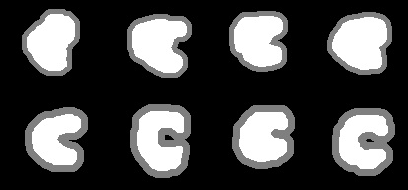
\includegraphics[width=85mm]{Figures/phantomwmgm} 
  \end{tabular}
\caption{The eight 2-D simulated images used for the initial parameter search.  These images  are available with the ANTS source distribution.}  
\label{fig:phantoms}
\end{figure}

\subsection{3-D NIREP Brain Image Normalization Evaluation}

The Non-Rigid Image Registration Project is a large-scale evaluation resource for deformable registration algorithms headed by Gary Christensen at the University of Iowa.  In addition to the development and distribution of the necessary software tools for algorithmic validation, this project includes the distribution of appropriate image data and corresponding segmentations.   One such database that has been made available is referred to as the ``NA0'' database consisting of 16 MR image volumes of normal adult human volunteers.  A brief demographic sketch of the NA0 database is as follows:  8 males with mean age of 32.5 $\pm$ 8.4 years (range of 25 to 48 years) and  8 females with mean age of 29.8 $\pm$ 5.8 years (range of 24 to 41).  

Following acquisition, each image was resampled and padded to isotropic voxel spacing of $0.7\times0.7\times0.7$ mm$^3$ and total size of $256 \times 300 \times 256$ voxels.
The cortex of each of the 16 MR image volumes was segmented into 32 regions \cite{Allen2002,Allen2003} using Brainvox which were later refined using manual editing.  

\begin{figure}
\centering
  \begin{tabular}{cc}
      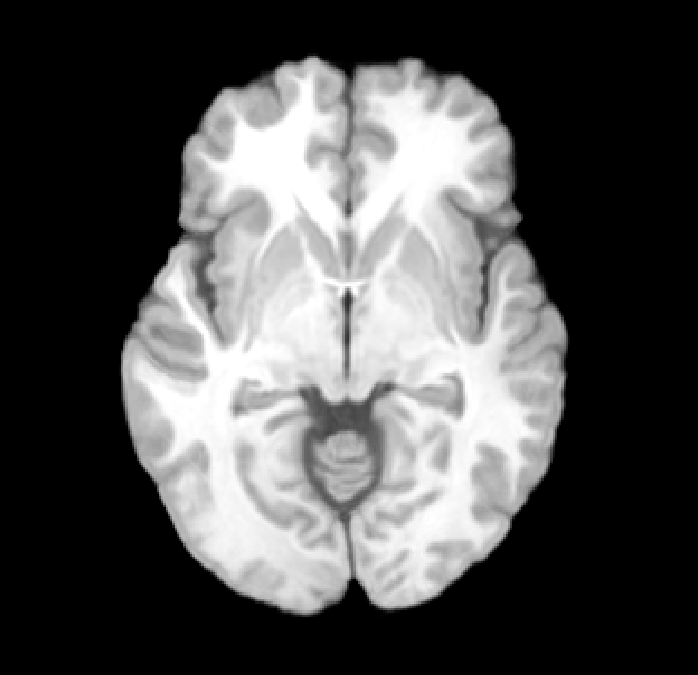
\includegraphics[width=40mm]{Figures/na01x_axial.png} &
      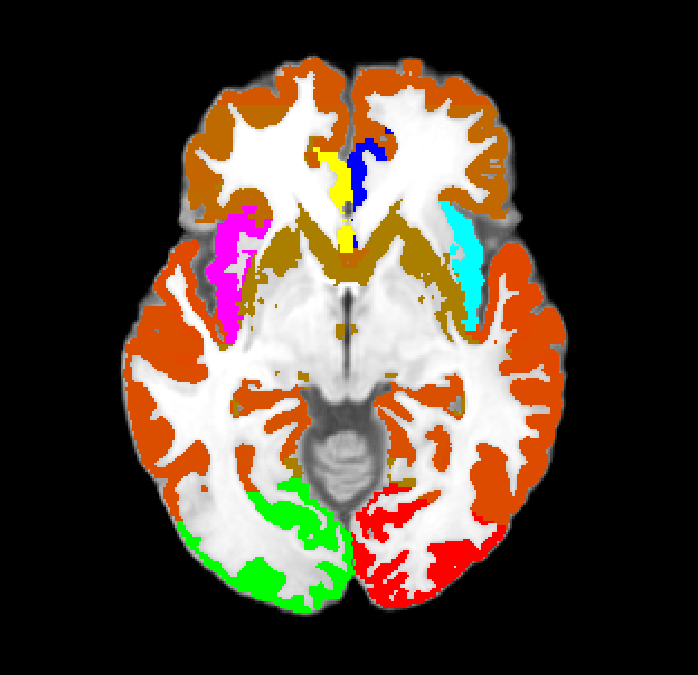
\includegraphics[width=40mm]{Figures/na01x_axial_labels.png} \\
      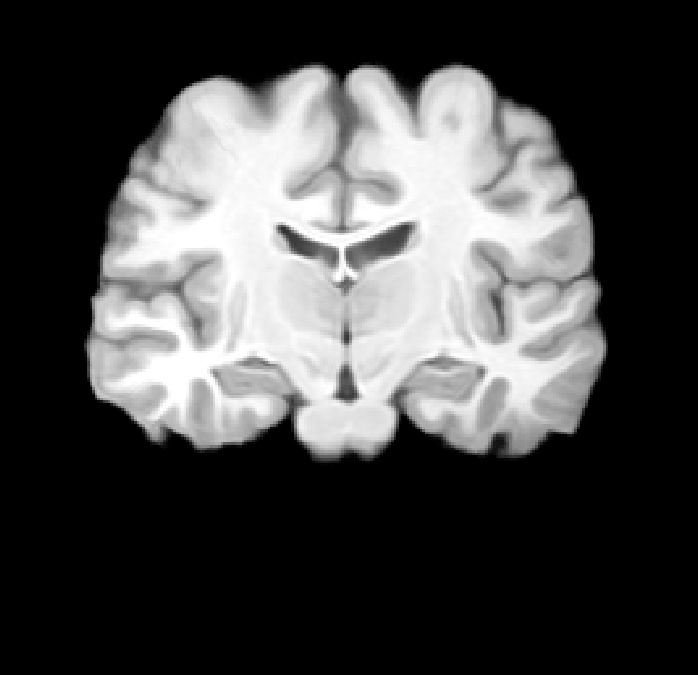
\includegraphics[width=40mm]{Figures/na01x_coronal.png} &
      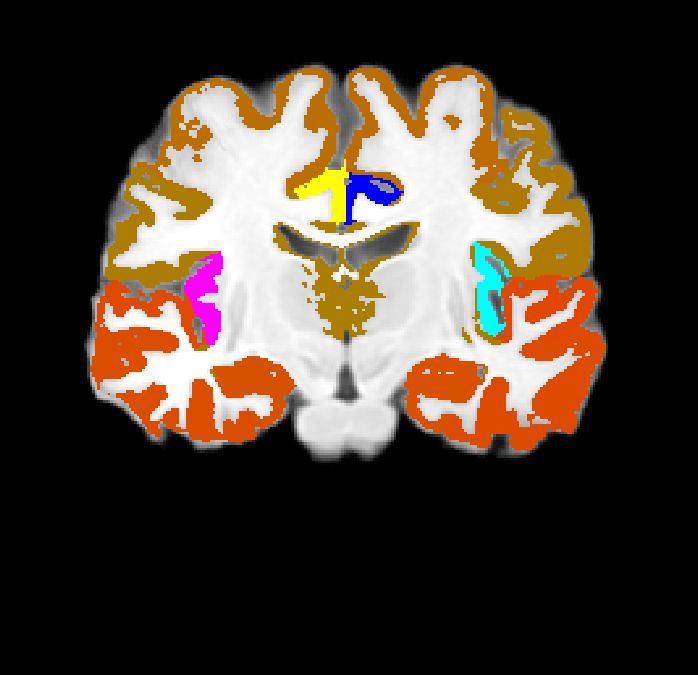
\includegraphics[width=40mm]{Figures/na01x_coronal_labels.png} \\
      \reflectbox{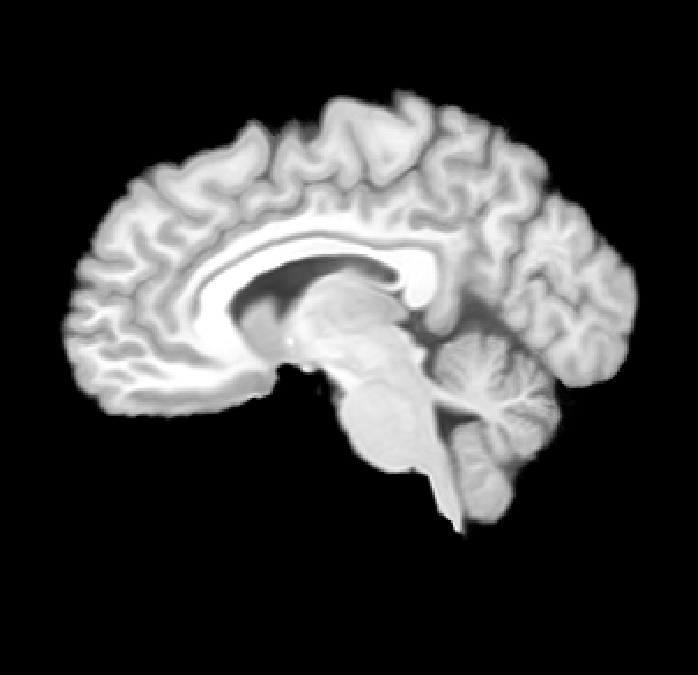
\includegraphics[width=40mm]{Figures/na01x_sagittal.png}} &
      \reflectbox{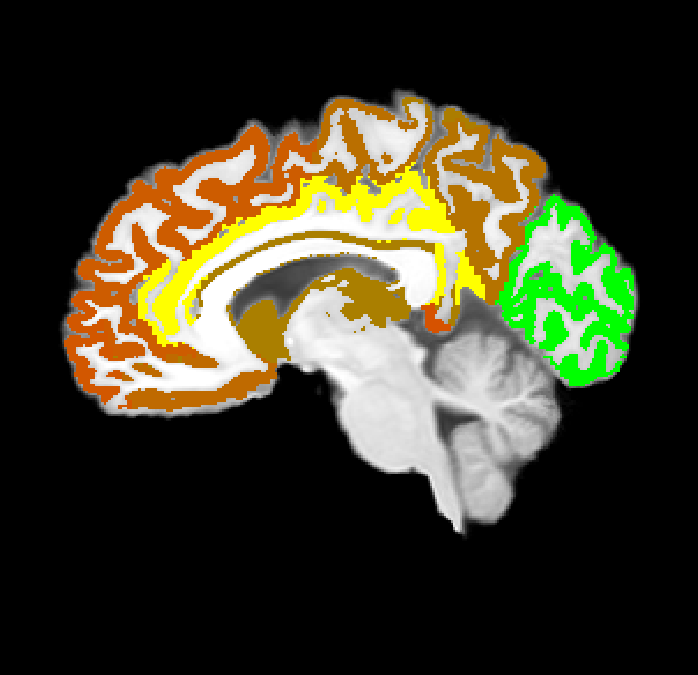
\includegraphics[width=40mm]{Figures/na01x_sagittal_labels.png}} \\
  \end{tabular}
\caption{Canonical image views of NA01 image from the NIREP data base (left column) and the corresponding segmentations (right column).  }  
\label{fig:na01x}
\end{figure}

Build template parallel with affine update .... scripts etc . 

\section{Discussion}

% use section* for acknowledgement
\section*{Acknowledgment}
ANTS is supported by Grant 1R01EB006266-01 from the National Institute Of Biomedical Imaging and Bioengineering and administered through the UCLA Center for Computational Biology.

\section{Additional ANTS Features}

\paragraph{Directly Manipulated Free-Form Deformation}
Another top performer in Klein's study \cite{Klein2009} was the Image
Registration Toolkit (IRTK) based on the research originally reported
in \cite{Rueckert1999} in which mutual information and a free-form
deformation (FFD) transformation model were used to analyze breast
deformation.  In ANTS we provide an implementation of a variant of the
well-known FFD transformation model for image registration known as
{\em directly manipulated free-form deformation} \cite{Tustison2009}.
The DMFFD model replaces the standard FFD gradient used in
\cite{Rueckert1999} with an intuitive preconditioned gradient to
overcome problematic energy topographies intrinsic with the
traditional approach.  DMFFD, in ANTS, is a regularization option 
as opposed to a specific registration method.  That is, we use the 
same transformation models and gradient descent strategies detailed above, 
but allow the DMFFD model to regularize the update or total deformation. 

For $n$-D images, the FFD (and DMFFD) transformational model, $\phi_{FFD}$, is defined as 
\begin{align}\label{eq:TFFD}
  \phi_{FFD} =  \sum_{i_1=1}^{M_1}\ldots\sum_{i_n=1}^{M_n} \mathbf{P}_{i_1, \ldots, i_n} \prod_{j=1}^nB_{i_j,d_j}(u_{j})     
\end{align}
where $\mathbf{P}_{i_1, \ldots, i_n}$ is an $n$-D grid of control points and $B_{i_j,d_j}(u_{j})$ is the B-spline in the $i_j^{th}$ direction of order $d_j$. 
The gradient of the image normalization energy, $\Pi$, with respect to the control points used during gradient-based optimization is easily calculated to be:
\begin{align} \label{eq:FFDgrad}
  \frac{\partial \Pi}{\partial \mathbf{P}_{i_1, \ldots, i_n}} =  \sum_{c=1}^{N_{\Omega}} \left(
  \frac{\partial \Pi_{\sim}}{\partial \phi} + \frac{\partial \Pi_{R}}{\partial \phi} 
  \right)_c \prod_{j=1}^nB_{i_j,d_j}(u^c_{j}),
\end{align}
which is the gradient used in \cite{Rueckert1999}.  In contrast, the DMFFD approach uses a preconditioned gradient given by:
\begin{align} \label{eq:DMFFDgrad}
 \frac{\partial \Pi}{\partial \mathbf{P}_{i_1, \ldots, i_n}} =& 
        \Bigg( \sum_{c=1}^{N_{\Omega}}   \left( \frac{\partial \Pi_{\sim}}{\partial \phi} + \frac{\partial \Pi_{R}}{\partial \phi}  \right)_c          \prod_{j=1}^n B_{i_j, d_j}(u^c_j)   \nonumber \\
  &  \cdot \frac{\prod_{j=1}^n B^2_{i_j, d_j}(u^c_j)}{\sum_{k_1=1}^{d_1+1}\ldots\sum_{k_n=1}^{d_n+1} \prod_{j=1}^n B^2_{k_j, d_j}(u^c_j)} \Bigg)  \nonumber \\
          &\cdot \left( \frac{1}{ \sum_{c=1}^{N_\Omega} \prod_{j=1}^n B^2_{i_j, d_j}(u^c_j)  } \right).
\end{align}
The difference between the two gradients is seen to reside strictly in terms of the B-spline shape functions which serve to normalize the DMFFD gradient in a unique fashion so as to minimize its susceptibility to hemstitching during the course of optimization.
The DMFFD approach, while available in ANTS, has not yet been exploited due to its relatively increased computational demands relative to the default regularization which is a fast Gaussian regularizer as in the Demons method.  
%A multi-resolution approach (\cite{Lee1997}) is included such that the B-spline mesh resolution is doubled at each stage of the optimization from a specified initial mesh resolution.  Also, all feasible B-spline orders are available (not just cubic).


\paragraph{Jensen-Havrda-Charvat-Tsallis Divergence}
Recent information theoretic approaches have been proposed for
point-set registration.  A previous open-source contribution
\cite{Tustison2009} generalizes the Jensen-Shannon divergence to the
Jensen-Havrda-Charvat-Tsallis (JCHT) divergence which permits a
fine-tuning of the divergence measure such that emphasis can vary
between robustness and sensitivity for application-speci�c tailoring
\cite{Tustison2009a}.

Each point-set is represented as a PDF via a Gaussian mixture model
(GMM).  Assuming $K$ point-sets denoted by $\{X_k, k \in
\{1,\ldots,K\}\}$, the $k^{th}$ point-set is denoted by $\{x^k_1,
\ldots, x^k_{|X_k|}\}$.  The corresponding $k^{th}$ PDF is calculated
from the $k^{th}$ point-set as
\begin{align}
  \mathbf{P}_k(s) = \frac{1}{|X_k|} \sum_{i=1}^{|X_k|} G( s; x^k_i,
  C^k_i )
\end{align}
where $G(s; x^k_i, C^k_i)$ is a normalized Gaussian with mean $x^k_i$
and covariance $C^k_i$ evaluated at $s$.  For each point, $x_i$, the
associated weighted covariance matrix, $C_{\mathcal{K}_i}$, is given
by
\begin{align} \label{eq:C}
  C_{\mathcal{K}_i} = \frac{ \sum_{x_j \in \mathcal{N}_i, x_j \neq
      x_i} \mathcal{K}(x_i; x_j) (x_i - x_j)^\mathrm{T} (x_i -
    x_j)}{\sum_{x_j \in \mathcal{N}_i, x_j \neq x_i} \mathcal{K}(x_i;
    x_j) }
\end{align}   
where $\mathcal{N}_i$ is the local neighborhood of the point $x_i$ and
$\mathcal{K}$ is a user-selected neighborhood weighting kernel.  We
use an isotropic Gaussian for $\mathcal{K}$ with variance
$\sigma_{\mathcal{K}_i}^2$ as well as a k-d tree structure for
efficient determination of $\mathcal{N}_i$ \cite{Berg2000}.
Calculation of the gradient requires the inverse of each covariance
matrix.  To avoid ill-conditioned covariance matrices, we use the
modified covariance $C_i = C_{\mathcal{K}_i} + \sigma_n^2 I$ where $I$
is the identity matrix and $\sigma_n$ is a parameter denoting added
isotropic Gaussian noise.

We designate the number of sample points generated for each of the $K$ probability density functions as $\{ M_1, \ldots, M_K \}$ and the $k^{th}$ set of points as $\{ s_1^k, \ldots, s_{M_k}^k \}$.  The JHCT divergence is then calculated using the $K$ sets of points and the formula
\begin{align} \label{eq:JHCT2}
  \mathrm{JHCT}_\alpha(&\mathbf{P}_1, \ldots, \mathbf{P}_K) =  \frac{1}{ 1-\alpha}  
  \nonumber \\
   &\left[\frac{1}{M} \left( \sum_{k=1}^K \sum_{j=1}^{M_k} \left[ \mathbf{P}^*(s_j^k) \right]^{\alpha-1} -1 \right)\right. \nonumber \\
   +&  \left. \frac{1}{N}\sum_{k=1}^K \frac{|X_k|}{M_k}   \left( \sum_{j=1}^{M_k} 
       \left[ \mathbf{P}_k(s_j^k) \right]^{\alpha-1} - 1 \right) \right]
\end{align}
where 
\begin{align}
\mathbf{P}^*(X) = \frac{1}{N}\sum_{k=1}^K \sum_{i=1}^{|X_k|} G(x;x_i^k, C_i^k), 
\end{align}
$N = \sum_{k = 1}^K |X_k|$, and $M = \sum_{k = 1}^K M_k$.
The prior weighting values are calculated from  $\gamma_k = |X_k|/N$ such that the larger point-sets are weighted more heavily.


\bibliographystyle{IEEEtran.bst}
\bibliography{./references.bib,ants,avantsAll}

\end{document}



